\documentclass[11pt, oneside]{article}   	% use "amsart" instead of "article" for AMSLaTeX format
\usepackage{geometry}                		% See geometry.pdf to learn the layout options. There are lots.
\geometry{letterpaper}                   		% ... or a4paper or a5paper or ... 
%\geometry{landscape}                		% Activate for for rotated page geometry
%\usepackage[parfill]{parskip}    		% Activate to begin paragraphs with an empty line rather than an indent
\usepackage{graphicx}				% Use pdf, png, jpg, or eps� with pdflatex; use eps in DVI mode
								% TeX will automatically convert eps --> pdf in pdflatex		
\usepackage{amssymb}
\usepackage{amsmath}

\title{Lines in $R^3$}
%\author{The Author}
%\section{}
% \subsection*{R code}
\date{}							% Activate to display a given date or no date

\graphicspath{{/Users/telliott_admin/Dropbox/Tex/png/}}

% \begin{center} 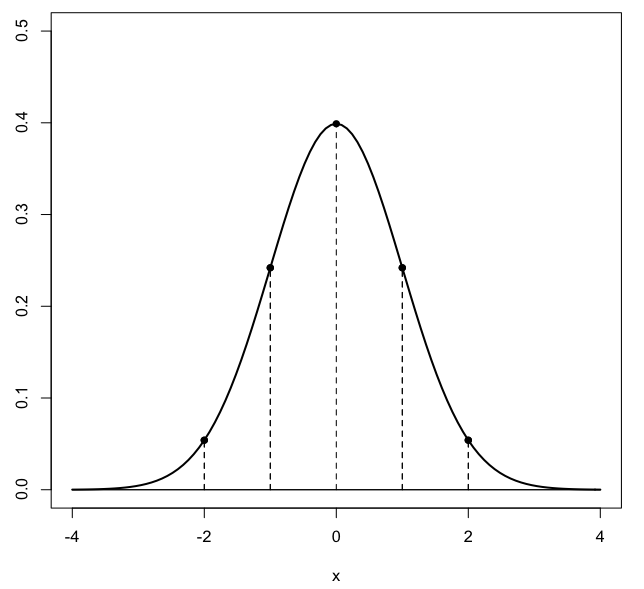
\includegraphics [scale=0.4] {gauss3.png} \end{center}
% \begin{bmatrix} a  &  b \\ c  &  d \end{bmatrix}
% \bigg |_

\begin{document}
\maketitle
\large
%\noindent
One way of specifying a line in 3D-space is as the intersection of two planes.  Another way is by giving a vector and a point in space.  Let's look at these in turn.
\noindent
Suppose we have the following two planes:
\[ x + y - z = 7 \]
\[2x - 3y + z = 3 \]

Since the $x,y,z$ terms are not related by a multiplicative constant, the planes are not parallel, so they will meet in a line, and the solutions consist of all the points on the line.  Let's find one solution, at $x=0$.  Then
\[ y - z = 7 \]
\[-3y + z = 3 \]
Adding
\[-2y = 10 \]
\[y = -5 \]
\[z = y - 7 = -12 \]
Our solution $P_0=(0,-5,-12)$.
Now find a second solution, at $z = -3$
\[ x + y = 4 \]
\[ 2x - 3y = 6 \]
Solving
\[ x = 4 - y \]
\[ 2(4-y) -3y = 6 \]
\[ 8 - 5y = 6 \]
\[ y = \frac{2}{5} \]
\[ x = \frac{18}{5} \]
The second point is $P_1 = (18/5, 2/5, -3)$.
Now we have two points on the line.  Its equation is 
\[ L = P_0 + t(P_1 - P_0) \]
\[ L = (0,-5,-12) + t(\frac{18}{5}, \frac{27}{5}, 9)\]
We can re-scale the vector that multiplies $t$ to have integer components (or length $1$, or whatever we wish).  Why not multiply by $5/9$?
\[ L = (0,-5,-12) + t(2, 3, 5)\]
There is another way to do this problem that might be a little easier.  Consider that the equation of the first plane gives its normal vector $n_1$ as
\[ n_1 =\ <1,1,-1> \]
Similarly the normal vector to the second plane is $n_2$
\[ n_2 =\ <2,-3,1> \]
Now, the vector that is parallel to the line of intersection is orthogonal to both $n_1$ and $n_2$  (Do you see why?)  So we compute the cross-product:
\[ n_1 \times n_2 = 
\begin{vmatrix} 
  i  &  j  &  k \\ 
  1  &  1 & -1 \\
  2  &  -3 & 1
\end{vmatrix}
\]
\[ = -2i -3j -5k \]
Multiplying by $-1$ gives what we obtained above.

\end{document}  